\documentclass{beamer}
\usepackage{hyperref}
\usepackage[T1]{fontenc}

% other packages
\usepackage{latexsym,amsmath,xcolor,multicol,booktabs,calligra}
\usepackage{graphicx,pstricks,listings,stackengine,amssymb}
\usepackage{algorithm}
\usepackage{algpseudocode}
\usefonttheme[onlymath]{serif}

\algnewcommand\algorithmicforeach{\textbf{for each}}
\algdef{S}[FOR]{ForEach}[1]{\algorithmicforeach\ #1\ \algorithmicdo}

\author{Capasso Giuseppe}
\title{Google Hashcode 2021 (World Finals)}
\subtitle{Software engineering at scale}
\institute{Algoritmi di ottimizzazione combinatoria e su rete}
\date{2023}
\usepackage{Tsinghua}

% defs
\def\cmd#1{\texttt{\color{red}\footnotesize $\backslash$#1}}
\def\env#1{\texttt{\color{blue}\footnotesize #1}}
\definecolor{deepblue}{rgb}{0,0,0.5}
\definecolor{deepred}{rgb}{0.6,0,0}
\definecolor{deepgreen}{rgb}{0,0.5,0}
\definecolor{halfgray}{gray}{0.55}

\lstset{
    basicstyle=\ttfamily\small,
    keywordstyle=\bfseries\color{deepblue},
    emphstyle=\ttfamily\color{deepred},    % Custom highlighting style
    stringstyle=\color{deepgreen},
    numbers=left,
    numberstyle=\small\color{halfgray},
    rulesepcolor=\color{red!20!green!20!blue!20},
    frame=shadowbox,
}


\begin{document}

\begin{frame}
    \titlepage
\end{frame}

\begin{frame}
    \tableofcontents[sectionstyle=show,subsectionstyle=show/shaded/hide,subsubsectionstyle=show/shaded/hide]
\end{frame}


\section{Descrizione del problema}

\begin{frame}{Problema}
    Schedulare un gruppo di $G$ ingegneri affinché siano implementate delle \textit{feature} all'interno di un \textit{datacenter} composto da $B$ server (o \textit{binary}) su cui sono in esecuzione $S$ servizi. Un server può ospitare più servizi, ma un servizio può risiedere su uno e un solo server.
    \begin{figure}[h]
        \centering
        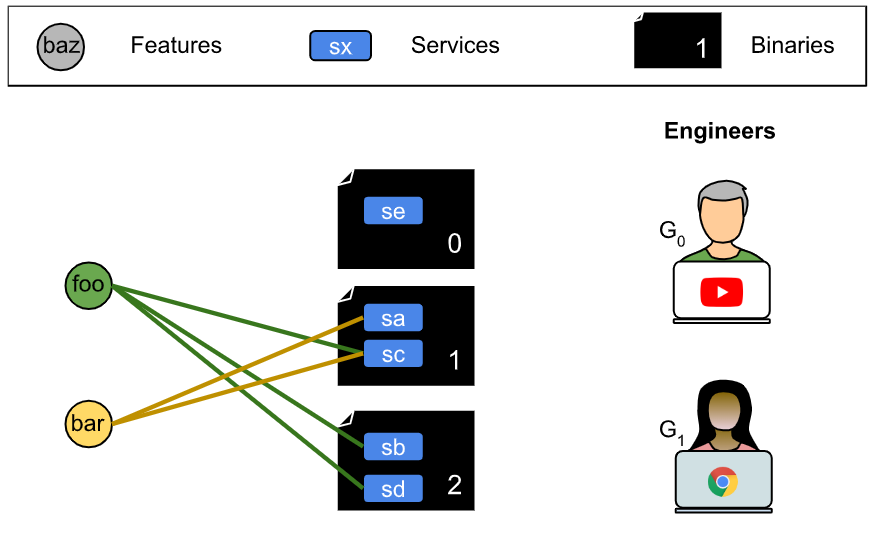
\includegraphics[height=.4\textheight]{pic/example.png}
    \end{figure}
    \textbf{Obiettivo:} massimizzare il numero di utenti soddisfatti
\end{frame}

\begin{frame}{Feature}
   Una feature è una funzionalità che, una volta implementata completamente, soddisfa un certo numero di clienti ed è caratterizzata da:
   \begin{itemize}
       \item Servizi in cui deve essere implementata
       \item Coefficiente di difficoltà $f_d$
       \item Numero di utenti soddisfatti $f_u$
   \end{itemize}
    \begin{figure}[h]
        \centering
        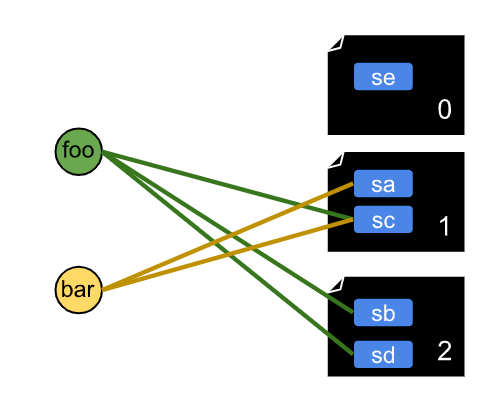
\includegraphics[height=.4\textheight]{pic/feature_binaries.png}
    \end{figure}    
\end{frame}

\begin{frame}{Scheduling}
   La schedulazione delle attività avviene con granularità giornaliera e varia su un arco temporale di $L$ giorni (dato in ingresso del problema)
    \begin{figure}[h]
        \centering
        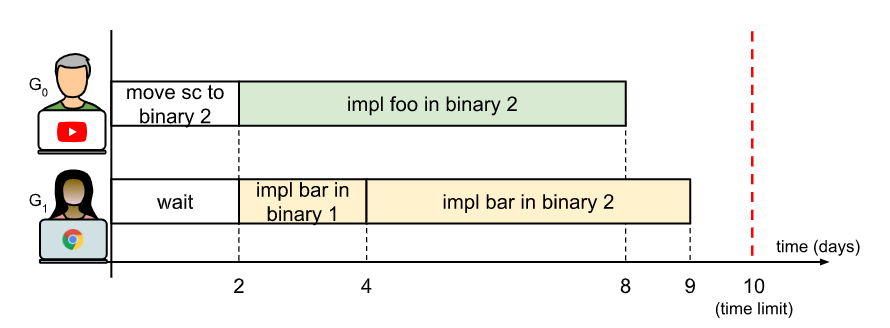
\includegraphics[height=.4\textheight]{pic/schedulazione.png}
    \end{figure}    
\end{frame}

\subsection{Attività}

\begin{frame}{Implementazione di una feature}
Un ingegnere può implementare una \textit{feature} $f \in F$ in un server $b \in B$. Questa azione comporta che tutti i servizi che risiedono sul server $b$, di cui necessita la \textit{feature}, la implementano. La durata dell'operazione è:
\begin{equation*}
    f_d + r_b + c_b
\end{equation*}
    \begin{itemize}
        \item $f_d$: coefficiente di difficoltà associato alla \textit{feature} $f$
        \item $r_b$: numero di servizi che risiedono sul server $b$
        \item $c_b$: numero di ingegneri al lavoro sul server $b$
    \end{itemize}
\end{frame}

\begin{frame}{Esempio}
     \begin{figure}[h]
        \centering
        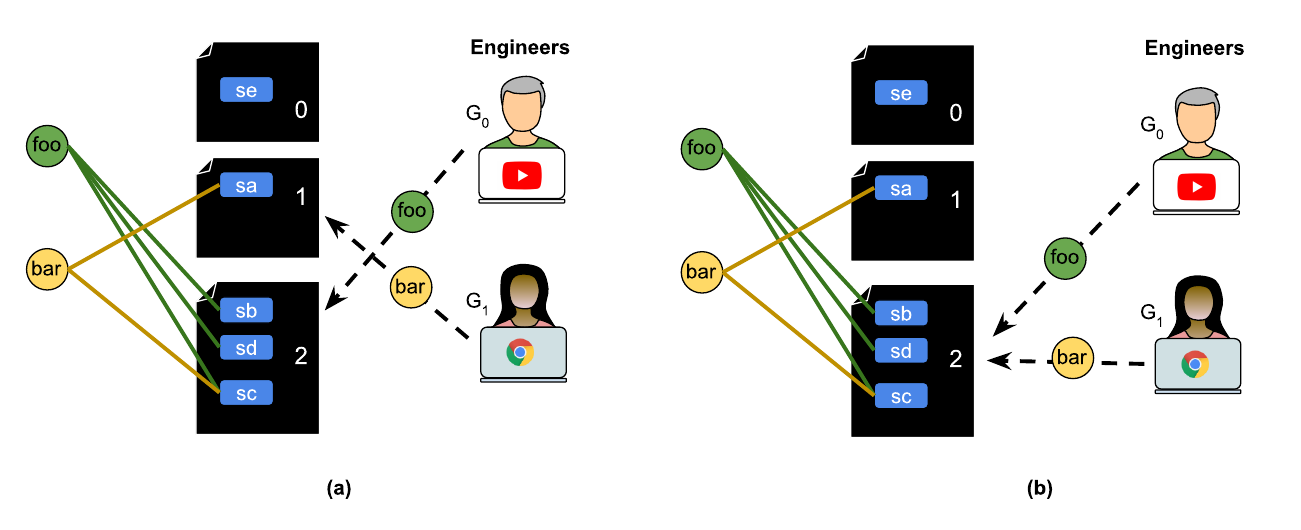
\includegraphics[height=.4\textheight]{pic/impl1.png}
    \end{figure}
\end{frame}

\begin{frame}{Migrazione di un servizio}
Un ingegnere può spostare un servizio $s \in S$ dal server in cui risiede $b_s$ ad un altro $b_t$. La durata dell'operazione è:
\begin{equation*}
   \max{(r_{bs}, r_{bt})}
\end{equation*}
    \begin{itemize}
        \item $r_{bs}$: numero di servizi presenti sul server $b_s$
        \item $r_{bt}$: numero di servizi presenti sul server $b_t$
    \end{itemize}
    \textbf{L'operazione è bloccante. Nessun ingegnere può lavorare su $b_s$ e $b_t$ mentre sono coinvolti in una migrazione}
\end{frame}

\begin{frame}{Esempio: migrazione di \textit{sc} sul server $2$}
    \begin{figure}[h]
       \centering
       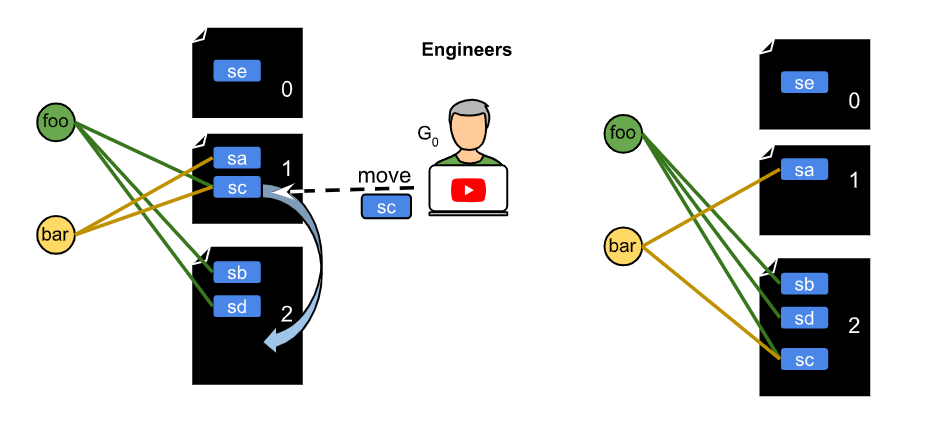
\includegraphics[width=.9\textwidth]{pic/migr_exa.png}
    \end{figure}    
\end{frame}

\begin{frame}{Creazione di un server}
Un ingegnere può creare un nuovo server all'interno del \textit{datacenter}. Questa operazione ha una durata costante $N$ specificata per ogni istanza del problema. 

\begin{figure}[h]
    \centering
    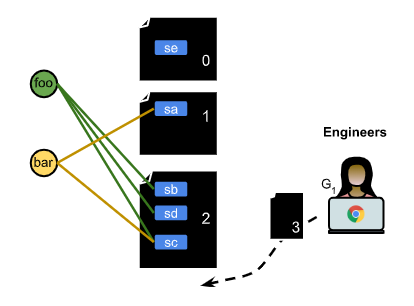
\includegraphics[height=.4\textwidth]{pic/new_server.png}
\end{figure}   
    
\end{frame}

\begin{frame}{Attesa}
Un ingegnere può aspettare non eseguendo nessuna delle altre attività per un numero di giorni inferiore a $L$.

\begin{figure}[h]
       \centering
       
\includegraphics[width=.7\textwidth]{pic/idle.png}
    \end{figure} 
    
\end{frame}

\section{Vincoli}

\begin{frame}{Vincoli principali}
\begin{itemize}
    \item Un ingegnere può effettuare una e una sola operazione al giorno
    \item Ingegneri diversi non possono implementare la stessa \textit{feature} sullo stesso server 
\end{itemize}
    \begin{figure}[h]
       \centering
       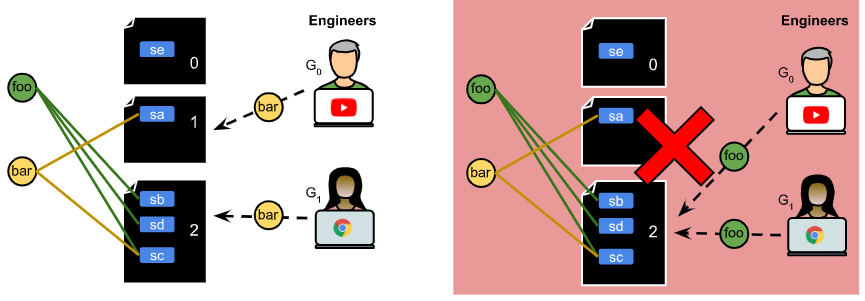
\includegraphics[width=.9\textwidth]{pic/vincolo.png}
    \end{figure} 
\end{frame}

\begin{frame}{Implementazione completa di una feature}
Una feature viene considerata completamente implementata se e solo se risulta implementata in tutti i servizi richiesti. In particolare, si definisce $B^f \subseteq B$ l'insieme dei server che servono ad implementare la \textit{feature} $f$.

Quindi una \textit{feature} implementata è valida se la durata dell'implementazione è inferiore a $L$. In simboli, detto $t^f_b$, il giorno in cui termina l'implementazione della \textit{feature} $f$ nel server $b$ questa risulta valida se e solo se:
\begin{equation*}
    t^f_b < L\; \forall b \in B^f
\end{equation*}

\end{frame}

\begin{frame}{Esempio}
    \begin{figure}[h]
        \centering
        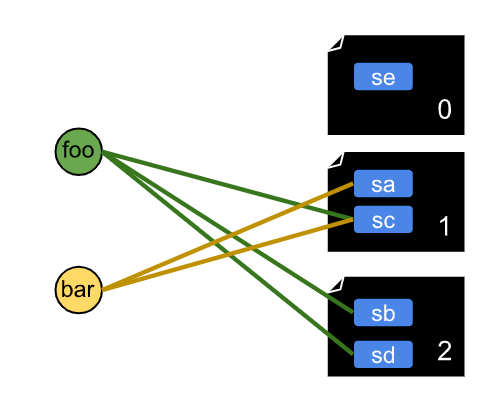
\includegraphics[height=.6\textheight]{pic/feature_binaries.png}
    \end{figure}  
\end{frame}

\begin{frame}{Calcolo del punteggio}
Posto $t^f = \max_{b \in B^f}{t^f_b}$ il tempo totale per l'implementazione della \textit{feature} $f \in F$, si assegna un punteggio $P_f$ pari a:
\begin{equation*}
    P_f = f_u \cdot \max{(0, L - t^f)}
\end{equation*}
con $f_u$ numero di utenti soddisfatti dall'implementazione della \textit{feature}.
\end{frame}

\section{Approcci utilizzati}

\subsection{Euristica greedy}

\begin{frame}{Spiegazione}
    L'euristica progettata si articola su 2 punti:
    \begin{itemize}
        \item Riduzione del numero di \textit{feature} parzialmente implementate
        \item Implementazione delle \textit{feature} di maggiore importanza
    \end{itemize}
\end{frame}

\begin{frame}{Riduzione del numero di feature parziali}
Questo punto viene implementato calcolando per ogni \textit{feature} $f$ l'insieme $B^f \subseteq B$ che corrisponde a quello dei server dove risiedono i servizi della \textit{feature}.

Per ogni feature $f$ da implementare, l'algoritmo effettua l'iterazione di tutti gli elementi dell'insieme $B^f$.

\end{frame}

\begin{frame}{Ordinamento delle \textit{feature}}
Si calcola il seguente fattore di priorità $p_f$:
\begin{equation*}
    p_f = \frac{f_{u}^{\alpha}} {|B^f| \cdot (|B^f| - 1 +  f_d)}
\end{equation*}
\begin{itemize}
    \item $f_u$: numero di utenti soddisfatti dalla \textit{feature}
    \item $|B^f|$: cardinalità dell'insieme di server su cui sono distribuiti i servizi da cui dipende la \textit{feature}
    \item $f_d$: difficoltà della \textit{feature}
    \item $\alpha$: parametro compreso tra 1 e 2 regolabile dall'utente che consente di ottenere un punteggio maggiore in alcune istanze. Ad esempio, nell'istanza $f$ con $\alpha = 1.8$ si raggiunge un punteggio migliore del $~10\%$ rispetto a $\alpha = 1.1$
\end{itemize}
\end{frame}

\begin{frame}{Spiegazione}
    Il coefficiente $p_f$ illustrato consente di:
    \begin{itemize}
        \item valorizzare le \textit{feature} che soddisfano un numero maggiore di clienti 
        \item penalizzare le \textit{feature} i cui servizi sono distribuiti su più server
        \item penalizzare le \textit{feature} più difficili da implementare
    \end{itemize}
\end{frame}


\begin{frame}{Pseudo-codice}
In una fase preliminare, per ogni \textit{feature}, si calcolano il coefficiente di priorità e i server su cui si trovano i servizi richiesti. Inoltre, si inizializzano le variabili di ciclo $f$ e $b$ per implementare ciascuna \textit{feature} in ogni server.

\begin{algorithm}[H]
\begin{algorithmic}[1]

\ForEach {$f \in F $}
    \State $f.binaries \gets calc\_servers(f.services)$ \Comment{Calcolo dei server }
    \State $f.prio \gets calc\_prio(f)$ \Comment{Calcolo del coefficiente di priorità}
\EndFor

\State $sort(F, key=prio)$ \Comment{Ordinamento delle feature per priorità}
\end{algorithmic}
\end{algorithm}


\end{frame}

\begin{frame}{Pseudo-codice - (contd.)}
\begin{algorithm}[H]
\begin{algorithmic}[1]
\State $f \gets 0$
\State $b \gets -1$
\ForEach{$l \in L$}
    \ForEach{$g \in G$}
        \If{$g.isAvailable(l)$}
            \State $b \gets b + 1$
            \If{$b = |B^f|$}
                \State $f \gets f+1$
                \State $b \gets 0$
            \EndIf
            \State $implement\_feature(g, f, b, l)$
        \EndIf
    \EndFor
\EndFor

\end{algorithmic}
\end{algorithm}
\end{frame}


\subsection{Euristica greedy migliorata}

\begin{frame}{Idea}
 L'idea principale è di utilizzare le operazioni di creazione server e migrazione servizi per ridurre il numero di ingegneri che lavora su una \textit{feature}.
 Rispetto alla \textit{greedy} precedente
\begin{itemize}
    \item Una \textit{feature} è implementata da un solo ingegnere
    \item Dati gli spostamenti dei servizi su server diversi, bisogna cambiare il fattore $p_f$ perché altrimenti bisognerebbe ricalcolarlo ad ogni iterazione visto che, potenzialmente, l'insieme $B^f \subseteq B$ cambia continuamente
    \item ogni ingegnere crea un server su cui viene spostata una parte dei servizi
\end{itemize}

\end{frame}

\begin{frame}{Nuovo fattore di priorità}
    Come detto in precedenza, per evitare una complessità computazionale elevata, invece di $B^f$ si definisce l'insieme $S^f \subseteq S$ che rappresenta l'insieme dei servizi necessari alla \textit{feature} $f \in F$:

    \begin{equation*}
    p'_f = \frac{f_{u}^{\alpha}} {|S^f| \cdot (|S^f| - 1 +  f_d)}
    \end{equation*}

    \begin{itemize}
    \item $f_u$: numero di utenti soddisfatti dalla \textit{feature}
    \item $|S^f|$: cardinalità dell'insieme di servizi necessari alla \textit{feature} $f$
    \item $f_d$: difficoltà della \textit{feature}
    \item $\alpha$: parametro compreso tra 1 e 2 regolabile dall'utente che consente di ottenere un punteggio maggiore in alcune istanze. Ad esempio, nell'istanza $f$ con $\alpha = 1.8$ si raggiunge un punteggio migliore del $~10\%$ rispetto a $\alpha = 1.1$
\end{itemize}

\end{frame}

\begin{frame}{Algoritmo (istanza $f$)}
\begin{itemize}
    \item Fase preliminare: ogni ingegnere crea un server in cui sposta devi servizi
    \item Fase implementativa: ogni ingegnere prende in carico una \textit{feature}, e sposta tutti i suoi servizi su un server per poi implementarla
    \item Fase di pulizia: l'ingegnere mette i servizi sui server iniziali
\end{itemize}
    
\end{frame}

\subsection{Approccio random}

\begin{frame}{Approccio random}
L'istanza $e$ è caratterizzata dal fatto di avere solo $2$ server, con $100$ \textit{feature} da implementare. In questo caso, i risultati dell'approccio random non sono tanto peggiori di quelli sviluppati con l'euristica greedy (circa 35M) con il vantaggio di essere di banale implementazione
    \begin{figure}[h]
        \centering
        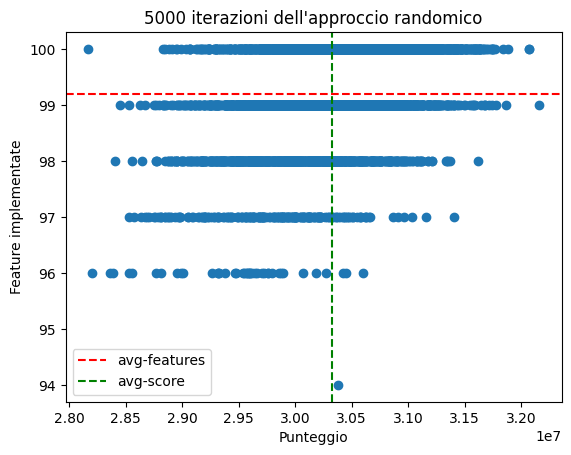
\includegraphics[height=.6\textheight]{pic/random.png}
    \end{figure}
\end{frame}

\begin{frame}{Pseudo-codice}
Scelta casuale delle attività:
\begin{algorithm}[H]
\begin{algorithmic}[1]
    \ForEach{$l \in L$}
    \ForEach{$g \in G$}
        \If{$g.isAvailable(l)$}
            \State $b \gets random.choice(servers)$
            \State $f \gets random.choice(features)$
            \State $implement\_feature(g, f, b, l)$
        \EndIf
    \EndFor
\EndFor
\end{algorithmic}
\end{algorithm}
\end{frame}

\section{Altri approcci (non implementati)}

\subsection{Job shop problem \cite{blazewicz2000disjunctive}}

\begin{frame}{Job shop problem}
Il problema può essere modellato come un \textit{Job Shop} noto in letteratura che prevede lo \textit{scheduling} di $n$ lavori su $m$ macchine.
\begin{itemize}
    \item Un lavoro è formato da più task
    \item I task in esecuzione non sono interrompibili
    \item Ogni task ha una durata fissa
\end{itemize}
\end{frame}

\begin{frame}{Job shop problem}
    \begin{itemize}
        \item $J$ lavori divisi in $a_{ij}$ task ($i-esimo$ task del lavoro $j-esimo$)
        \item $M$ macchine su cui effettuare i lavori
        \item Ad ogni task $a_{ij}$ è associata una coppia $(m_{ij},p_{ij})$ (il task deve essere completato sulla macchina $m \in M$ con una durata $p_{ij}$)
    \end{itemize}
\end{frame}

\begin{frame}{Modellazione mediante un grafo}
    Questo problema viene modellato attraverso un grafo disgiuntivo $G = (V, C \cup D)$:
    \begin{itemize}
        \item V: \textit{task} $a_{ij}$, con l'aggiunta di nodi fittizi di sorgenti e destinazione
        \item C: archi che interconnettono i \textit{task} di un singolo \textit{job}
        \item D: insieme di archi che interconnettono i \textit{task} processati sulla stessa macchina
    \end{itemize}
\end{frame}

\begin{frame}{Modellazione su un grafo}
    \begin{figure}[h]
        \centering
        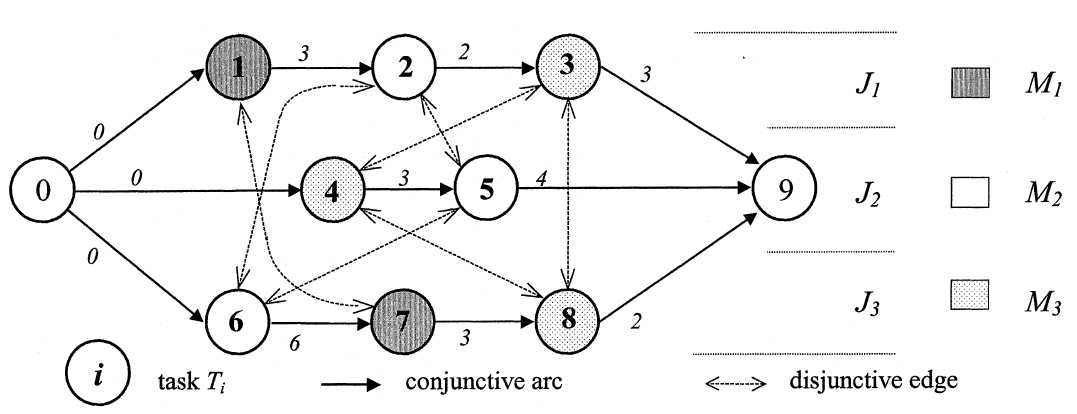
\includegraphics[height=.4\textheight]{pic/disjuntive_graph.png}
    \end{figure}
\end{frame}

\begin{frame}{Archi disgiuntivi}
Gli archi disgiuntivi possono essere raggruppati in \textit{clique} indipendenti $D_k$ con $D=\bigcup_{k \in M} D_k$ in cui è possibile identificare la schedulazione su una singola macchina.

    \begin{figure}[h]
        \centering
        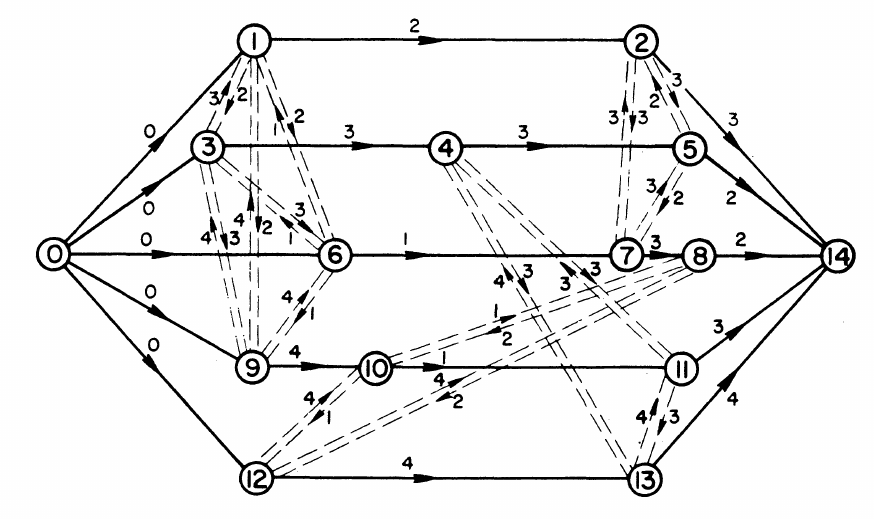
\includegraphics[height=.6\textheight]{pic/clique.png}
    \end{figure}
    
\end{frame}

\begin{frame}{Soluzione}
Una soluzione ammissibile può essere trovata orientando gli archi dei vincoli di disgiunzione e trovando un grafo aciclico. Inoltre, si dimostra che una soluzione ottima è composta trovando il percorso minimo dalla sorgente alla destinazione.
\begin{figure}[h]
        \centering
        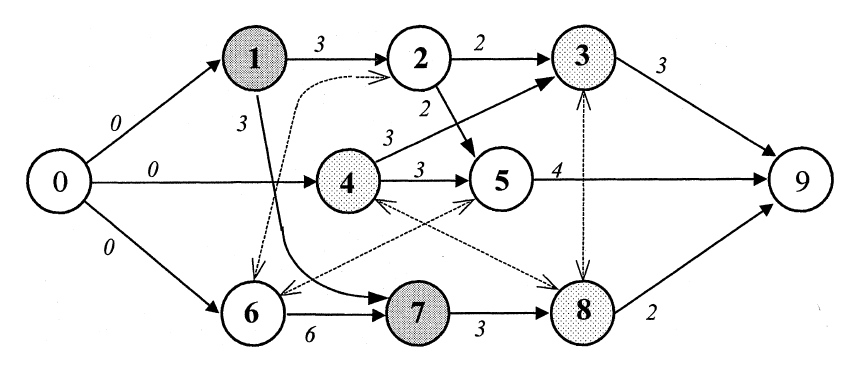
\includegraphics[height=.4\textheight]{pic/solution.png}
    \end{figure}
\end{frame}

\begin{frame}{Euristica bottleneck shifting \cite{adams1988shifting}}
    Al contrario delle euristiche greedy, viene sacrificata complessità computazionale per avere delle soluzioni migliori:
    \begin{itemize}
        \item Viene risolto il problema dello \textit{scheduling} su una singola macchina ripetutamente
        \item Ad ogni iterazione si effettua il sequenziamento di una macchina e si ritorna sulle precedenti per ottimizzare la schedulazione
        \item La macchina scelta è che causa \textbf{\textit{bottlneck}}
    \end{itemize}
\end{frame}

\begin{frame}{Bottleneck}
    Dato un insieme di macchine $M_0$ già schedulate, la macchina $m_k\; con\; k \in M\setminus M_0$ che provoca \textit{bottleneck} è quella che massimizza la \textit{lateness}.
\begin{equation*}
    \max v(k,M_0)\; k \in M\setminus M_0
\end{equation*}
Dove con $v(k, M_0)$ si indica una soluzione al problema di \textit{scheduling} su singola macchina.\\
Risolvere il bottleneck significa minimizzare la \textit{lateness} e quindi risolvere un problema di \textit{min-max}
    
\end{frame}

\begin{frame}{Applicazione al problema corrente}
La formulazione si può applicare al problema
\begin{itemize}
    \item I \textit{task} di un \textit{job} corrispondono all'implementazione di una \textit{feature} all'interno di un server (dove risiedono i servizi necessari)
    \item Le macchine corrispondono agli ingegneri che possono effettuare l'azione di implementazione di una \textit{feature} su un determinato server
    \item Il tempo di completamento di una \textit{feature} può essere calcolato staticamente scegliendo il caso peggiore (quello in cui tutti gli ingegneri sono al lavoro sullo stesso server)
\end{itemize}
\end{frame}

\begin{frame}{Altre approcci risolutivi}
    \begin{itemize}
        \item \textbf{Ricerca locale}: con un'euristica di tipo \textit{tabu-search} si potrebbe partire da una schedulazione ammissibile e cercare di migliorarla sostituendo alla mossa di "implementazione" una di "migrazione"
        \item \textbf{Algoritmi genetici}: partendo da una popolazione di soluzioni generata causalmente, si possono generare delle soluzioni ammissibili non solo implementando una \textit{feature} in un server, ma usando anche le altre mosse a disposizione con un operatore di mutazione
        \item \textbf{Vehicle routing}: ad ogni ingegnere viene associato un cluster. Ogni nodo rappresenta una mossa che l'ingegnere può effettuare
    \end{itemize}
\end{frame}

\section{Bibliografia}

\begin{frame}[allowframebreaks]
    \bibliography{ref}
    \bibliographystyle{alpha}
\end{frame}

\begin{frame}
    \begin{center}
        {\Huge Codice}
    \end{center}
\end{frame}

\end{document}